\documentclass{article}
\usepackage{fancyhdr} % for pretty formatting
\usepackage{amsmath} % for matrices
\usepackage{amssymb} % for bold text
\usepackage{pgfplots} % for graphs
\usepackage{hyperref} % for hyperlinks
\pgfplotsset{compat=1.18}
\usepackage{enumitem} % for custom lists

\usepackage{lipsum} % For dummy text
\usepackage{cite} % For citations

\usepackage{tcolorbox} % Required for tcolorbox

\newtcolorbox{asidebox}{
    colback=gray!10, % Background color
    colframe=gray!50, % Frame color
    boxsep=5pt, % Padding
    arc=4pt, % Rounded corners
    title=Aside, % Optional title for the aside
    fonttitle=\bfseries, % Title font style
} % for Asides

\pagestyle{fancy}
\fancyhf{} % Clear all header and footer fields

\lhead{Joshua Dunne}
\rhead{\thepage} % Displays the current page number
\lfoot{MATH620}
\rfoot{Unit 3}
\cfoot{Task 2}

\begin{document}
\section{Given}
    We're given a set of letters that align mostly with a set of grid coordinates.
    We are also given a selection of possible resultant transformations
\section{Wanted}
    We want to find the matching transformation that maps the original set of letters to the new set of letters.
\section{Answer}
    \paragraph{Approach}
        We can start by making a few important observations
        \begin{enumerate}
            \item The letters are made up of lines which are made up of points
            \item Each point has a coordinate in the form of (x,y)
            \item Each transformation will affect the coordinates of each point in a specific way
            \item By applying each transformation to the original coordinates, we can see which one results in the new coordinates
            \item The transformation that results in the new coordinates is the correct one
        \end{enumerate}
    \paragraph{Solution}
        Lets represent the points of the original letters as a composite matrix
        \[
            \begin{bmatrix}
                0&0&0&x_4&x_5&...&x_{27}\\
                0&3&3&y_4&y_5&...&y_{27}\\
            \end{bmatrix}
        \]
        And multiply that along with our imposed transformation $A=\begin{bmatrix}1&\frac{1}{3}\\0&\frac{4}{3}\end{bmatrix}$.
        \[
            \begin{bmatrix}
                0&0&0&x_4&x_5&...&x_{27}\\
                0&3&3&y_4&y_5&...&y_{27}\\
            \end{bmatrix}
            \begin{bmatrix}1&\frac{1}{3}\\0&\frac{4}{3}\end{bmatrix}
            =
            \begin{bmatrix} % This is incorrect. The transformation is applied to the coordinates, not multiplied by the matrix of coordinates.
                0&0&0&x_4&x_5&...&x_{27}\\ % The result of the transformation should be a new set of coordinates.
                0&3&3&y_4&y_5&...&y_{27}\\ % This matrix multiplication is not the correct way to apply a transformation to a set of points.
            \end{bmatrix}
        \]
        What results is a new set of coordinates that match the new set of letters.
        Therefore the transformation that maps the original set of letters to the new set of letters is $B$.
        \begin{asidebox}
            We could also arive at this conclusion by eliminating the other options.
            For example, others could not have been arrived at by transformation as they
            had characteristics, like $(0, 0) \not\rightarrow (0, 0)$
        \end{asidebox}
    \section{Illustration}
        Happily, through this method, and alot of punching at a calculator,
        we can see that the transformation $B$ does indeed map the original set of letters to the new set of letters.
        \\
        \begin{center}   
        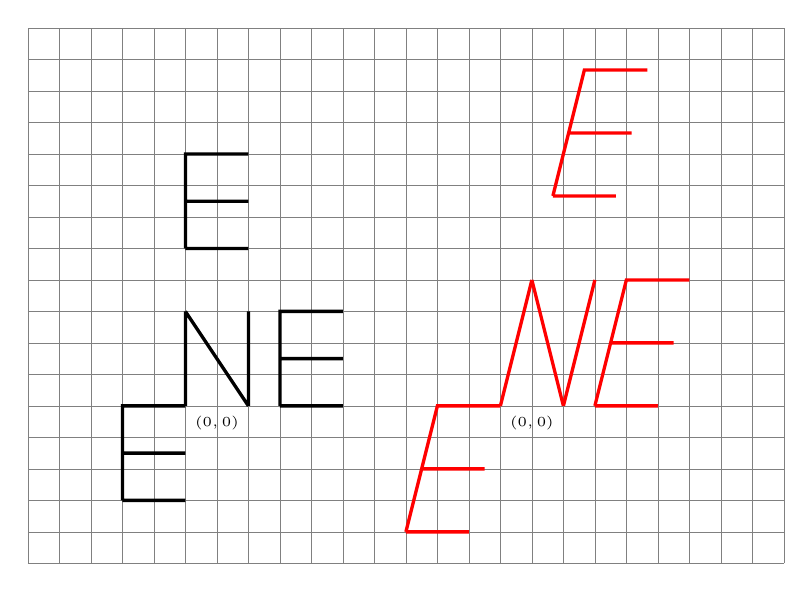
\begin{tikzpicture}[
            every node/.style={font=\tiny},
            scale=0.4 % Adjusted scale to fit a reasonable paper size, you can change this
        ]

            % 1. Draw the Grid
            % The image covers from x=-2 to x=8 and y=-1 to y=7, so a 10x8 grid is sufficient.
            \draw[step=1.0, gray, very thin] (-5, -5) grid (19, 12);

            % 2. Draw the Axes and Origin Label
            % Label the origin as shown in the image
            \node[below right] at (0,0) {$(0,0)$};
            
            % 3. Draw the "ENE" Shape (using a thicker line style)
            \draw[very thick]
                % Bottom-Left E
                (0, 0) -- (-2, 0) -- (-2, -3) % Left Bar of E
                (-2, -1.5) -- (0, -1.5) % Middle Bar of E
                (-2, -3) -- (0, -3) % Bottom Bar of E
                
                % Center N
                (0, 0) -- (0, 3) % Left Bar of N
                (0, 3) -- (2, 0) % Diagonal Bar of N
                (2, 0) -- (2, 3) % Right Bar of N
                
                % Top E
                (0, 5) -- (0, 8) -- (2, 8) % Vertical
                (0, 6.5) -- (2, 6.5) % Middle Bar
                (0, 5) -- (2, 5) % Bottom
                
                % Right E
                (3, 0) -- (3, 3) -- (5, 3) % Vertical
                (3, 1.5) -- (5, 1.5) % Middle Bar
                (3, 0) -- (5, 0); % Bottom Bar    % Transformed ENE

            \node[below right] at (10,0) {$(0,0)$};
            \draw[very thick, red]
                % Bottom-Left E
                (10, 0) -- (8, 0) -- (7, -4) % Left Bar of E
                (7.5, -2) -- (9.5, -2) % Middle Bar of E
                (7, -4) -- (9, -4) % Bottom Bar of E
                
                % Center N
                (10, 0) -- (11, 4) % Left Bar of N
                (11, 4) -- (12, 0) % Diagonal Bar of N
                (12, 0) -- (13, 4) % Right Bar of N
                
                % Top E
                (35/3, 20/3) -- (38/3, 32/3) -- (44/3, 32/3) % Vertical
                (12.1667, 8.6667) -- (14.1667, 8.6667) % Middle Bar
                (35/3, 20/3) -- (41/3, 20/3) % Bottom
                
                % Right E
                (13, 0) -- (14, 4) -- (16, 4) % Vertical
                (13.5, 2) -- (15.5, 2) % Middle Bar
                (13, 0) -- (15, 0); % Bottom Bar


        \end{tikzpicture}
        \end{center}
\end{document}